% -*- mode: noweb; noweb-default-code-mode: R-mode; -*-
\documentclass[11pt]{article}
%% Set my margins
\setlength{\oddsidemargin}{0.0truein}
\setlength{\evensidemargin}{0.0truein}
\setlength{\textwidth}{6.5truein}
\setlength{\topmargin}{0.0truein}
\setlength{\textheight}{9.0truein}
\setlength{\headsep}{0.0truein}
\setlength{\headheight}{0.0truein}
\setlength{\topskip}{0pt}
%% End of margins

%%\pagestyle{myheadings}
%%\markboth{$Date$\hfil$Revision$}{\thepage}

\usepackage[pdftex,
bookmarks,
bookmarksopen,
pdfauthor={Zequn Sun, Wei Wei and Dongjun Chung},
pdftitle={PICS Vignette}]
{hyperref}

% \usepackage{fullpage}
% \usepackage{pdflscape}

\title{An Introduction to the `\texttt{PICS}' Package, Version 1.0}
\author{ Zequn Sun,Wei Wei and Dongjun Chung\\
Department of Public Health Sciences, Medical University of South Carolina (MUSC),\\
  Charleston, SC, 29425.}


\date{\today}



\usepackage{Sweave}
\begin{document}
\Sconcordance{concordance:PICS-example.tex:PICS-example.Rnw:%
1 36 1 1 0 23 1 1 4 1 2 4 0 1 2 16 1 1 2 1 0 1 1 10 0 1 1 5 0 1 1 5 0 1 %
1 12 0 1 2 4 1 1 2 1 0 1 1 10 0 1 2 15 1 1 2 4 0 1 3 11 0 1 2 18 1 1 2 %
1 0 1 1 16 0 1 2 17 1 1 2 4 0 1 2 3 1 2 2 8 1 1 2 1 0 1 1 18 0 1 2 4 1 %
1 2 26 0 2 2 4 0 1 2 5 1 2 2 7 1 1 2 4 0 1 2 3 1 2 2 16 1}

%\VignetteIndexEntry{PICS}
%\VignetteKeywords{PICS}
%\VignettePackage{PICS}
%\VignetteEncoding{UTF-8}
\maketitle

\section{Overview}

This vignette provides basic information about the
\texttt{PICS} \cite{PICS} package. PICS stands for ``Pathway-guided Identification of Cancer Subtypes''.
The proposed approach improves identification of molecularly-defined subgroups of cancer patients by utilizing information from pathway databases in the following four aspects.

(1) Integration of genomic data at the pathway-level improves robustness and stability in identification of cancer subgroups and driver molecular features;

(2) Summarizing multiple genes and genomic platforms at the pathway-level can potentially improve statistical power to identify important driver pathways because moderate signals in multiple genes can be aggregated;

(3) In \texttt{PICS}, we consider this ``cooperation'' or ``interaction'' between pathways, instead assuming that each pathway operates independently during the cancer progression, which may be unrealistic;

(4) \texttt{PICS} allows simultaneous inference in multiple biological layers (pathway clusters, pathways, and genes) within a statistically rigorous and unified framework without any additional laborious downstream analysis.

The package can be loaded with the command:


\begin{Schunk}
\begin{Sinput}
R> library("PICS")
\end{Sinput}
\end{Schunk}

\section{Input Data}

The package requires that the response consist of 4 components:
(1) z-scores in the form of a either data frame or matrix; and
(2) survival time and censoring indicator in the form of vectors; and
(3) pathway information is in the form of a list where gene names are included in pathway lists respectively.

The Cancer Genome Atlas (TCGA) will be used to illustrate the `\texttt{PICS}' package.
The TCGA data was downloaded from the cBio Portal (http://www.cbioportal.org/) using the R package `\texttt{cgdsr}', and we used z scores for the mRNA expression data.

The `\texttt{PICS}' package provided an example data `\texttt{TCGA}'. The `\texttt{TCGA}' is a list object with four elements, including the `\texttt{geneexpr}' data frame of z scores for the mRNA expression, the `\texttt{t}' vector of the survival time, the `\texttt{d}' vector of the survival status indicator, and the `\texttt{pathList}' list of the pathway information. The `\texttt{pathList}' has four elements, each of which contains names of genes belonging to each pathway. Z scores for the mRNA expression data of 389 genes are provided for 50 randomly selected high-grade serous ovarian cancer patients, along with survival times and censoring statuses.

This dataset can be loaded as follows:

\begin{Schunk}
\begin{Sinput}
R> data(TCGA)
R> TCGA$geneexpr[1:5,1:5]
\end{Sinput}
\begin{Soutput}
        ACLY        ACO1       ACO2         CS       DLAT
1 -2.2410125 -0.48445531 -1.6346455  0.1378804 -3.5310321
2 -2.1301362  0.82116427 -0.9533701  0.6213512  0.6689948
3 -2.9122727 -0.08790649 -1.0975096 -0.2454025 -0.9433900
4 -1.1721514 -0.24249825 -0.7212639  0.1842386 -0.6188785
5  0.5383438  0.98012739 -0.7396043 -0.0699680  1.9573767
\end{Soutput}
\begin{Sinput}
R> TCGA$t[1:5]
\end{Sinput}
\begin{Soutput}
[1] 43.89 40.97 49.12  2.00 46.59
\end{Soutput}
\begin{Sinput}
R> TCGA$d[1:5]
\end{Sinput}
\begin{Soutput}
[1] 1 1 0 1 0
\end{Soutput}
\begin{Sinput}
R> TCGA$pathList[1]
\end{Sinput}
\begin{Soutput}
$KEGG_CITRATE_CYCLE_TCA_CYCLE
 [1] "IDH3B"     "DLST"      "PCK2"      "CS"        "PDHB"      "PCK1"     
 [7] "PDHA1"     "LOC642502" "PDHA2"     "LOC283398" "FH"        "SDHD"     
[13] "OGDH"      "SDHB"      "IDH3A"     "SDHC"      "IDH2"      "IDH1"     
[19] "ACO1"      "ACLY"      "MDH2"      "DLD"       "MDH1"      "DLAT"     
[25] "OGDHL"     "PC"        "SDHA"      "SUCLG1"    "SUCLA2"    "SUCLG2"   
[31] "IDH3G"     "ACO2"     
\end{Soutput}
\end{Schunk}

\section{Pre-filtering}

To refine the candidate set of genes, we first conduct a supervised pre-filtering by fitting a Cox regression model of each mRNA expression measure on patient survival in the TCGA dataset. Only the gene expressions associated with patient survival at p-values smaller than a pre-specified cut-off are included in the subsequent analysis. By default, p = 0.5 is used as cut-off point.

\begin{Schunk}
\begin{Sinput}
R> prefilter.results <- prefilter(data=TCGA$geneexpr, time=TCGA$t, status=TCGA$d, plist=TCGA$pathList)
R> prefilter.results
\end{Sinput}
\begin{Soutput}
Summary: Pre-filtering results (class: Prefiltered)
--------------------------------------------------
Number of genes before prefiltering: 389
Number of genes after prefiltering: 213
--------------------------------------------------
\end{Soutput}
\end{Schunk}

\section{Gene Selection}
In order to select key genes associated with patient survivals and effectively summarize them by taking into account correlation among them, we fit a sparse partial least squares (SPLS) Cox regression model \cite{SPLS} of patient survivals on gene expression measurements for each pathway.

Using the `\texttt{prefilter.results}', gene-level analysis result can be generated with `\texttt{selectGene}' function.

\begin{Schunk}
\begin{Sinput}
R> gene.results <- selectGene(prefilter.results)
\end{Sinput}
\end{Schunk}
\begin{Schunk}
\begin{Sinput}
R> gene.results
\end{Sinput}
\begin{Soutput}
Summary: Gene-level analysis results (class: FitGene)
--------------------------------------------------
Number of prefiltered genes: 213
Number of selected genes: 132
--------------------------------------------------
\end{Soutput}
\end{Schunk}

The list of the SPLS regression coefficients of cancer related genes can be generated using the function \texttt{coef()}.

\begin{Schunk}
\begin{Sinput}
R> head(coef(gene.results)[[1]])
\end{Sinput}
\begin{Soutput}
  gene       coef
1 ACLY  0.0000000
2   CS  0.0000000
3 DLAT  0.0000000
4  DLD  0.0000000
5 MDH1 -0.3560516
6 PCK1 -0.1988449
\end{Soutput}
\end{Schunk}

There are two main tuning parameters: `\texttt{eta}' represents
the sparsity tuning parameter and `\texttt{K}'
is the number of hidden (latent) components. Parameters can be chosen by ($v$-fold)
cross-validation. The user can search the range for these parameters and
the cross-validation procedure
searches within these ranges. Note that `\texttt{eta}' should have a value between 0 and 1. `\texttt{K}'
is integer valued and can range between
1 and $ min \left\{ p, (v-1) n / v \right\} $, where $p$ is the number of genes and $n$ is the sample size. For example, if 10-fold cross-validation is used (default), `\texttt{K}' should be smaller than $ min \left\{ p, 0.9 n \right\} $. For the TCGA data, we set fold as 5, `\texttt{K}' as 5, and search for `\texttt{eta}' between 0.1 and 0.9 with the following command:


\section{Pathway Selection}

Next, in order to identify a parsimonious set of pathways associated with patient survivals, we fit a LASSO-penalized Cox regression \cite{LASSO} on latent components derived from all the pathways.
Specifically, a pathway was selected if at least one of its latent components had non-zero LASSO coefficient estimate.

This approach has the following two strengths:
First, the latent components generated from the SPLS step preserve pathway structure and also reflect correlation among genes and their association with survival outcomes. Second, this approach can potentially improve the stability of estimation in the subsequent analysis.

Using the `\texttt{gene.results}', pathway-level analysis result can be generated with `\texttt{selectPath}' function.

\begin{Schunk}
\begin{Sinput}
R> path.results <- selectPath(gene.results)
R> path.results
\end{Sinput}
\begin{Soutput}
Summary: Pathway-level analysis results (class: FitPath)
--------------------------------------------------
Number of all pathways: 4
Number of selected pathways: 4

List of selected pathways:
	KEGG_CITRATE_CYCLE_TCA_CYCLE:
	KEGG_MAPK_SIGNALING_PATHWAY:
	KEGG_TGF_BETA_SIGNALING_PATHWAY:
	KEGG_THYROID_CANCER:
--------------------------------------------------
\end{Soutput}
\end{Schunk}

LASSO regression coefficients of cancer related pathways can be generated using the function \texttt{coef()}.

\begin{Schunk}
\begin{Sinput}
R> head(coef(path.results))
\end{Sinput}
\begin{Soutput}
                          pathway       coef
1    KEGG_CITRATE_CYCLE_TCA_CYCLE 0.44388849
2    KEGG_CITRATE_CYCLE_TCA_CYCLE 0.00000000
3    KEGG_CITRATE_CYCLE_TCA_CYCLE 0.00000000
4    KEGG_CITRATE_CYCLE_TCA_CYCLE 0.00000000
5     KEGG_MAPK_SIGNALING_PATHWAY 0.08378862
6 KEGG_TGF_BETA_SIGNALING_PATHWAY 0.37094205
\end{Soutput}
\end{Schunk}

Hazard ratio plot associated with each latent component in selected pathways can be generated using the function \texttt{plot()} with the argument \texttt{type="{}HR"{}}.

\begin{Schunk}
\begin{Sinput}
R> plot(path.results, type="HR")
\end{Sinput}
\end{Schunk}

Figure 1 shows the hazard ratio (HR) associated with each latent component in the pathways selected by the \texttt{PICS}.
Based on the TCGA data, pathways with the largest effect on survival (HR $\geq 1.15$) are \texttt{KEGG\_CITRATE\_CYCLE\_TCA\_CYCLE} and \texttt{KEGG\_TGF\_BETA\_SIGNALING\_PATHWAY} pathways.

\begin{figure}[tbh]
\begin{center}
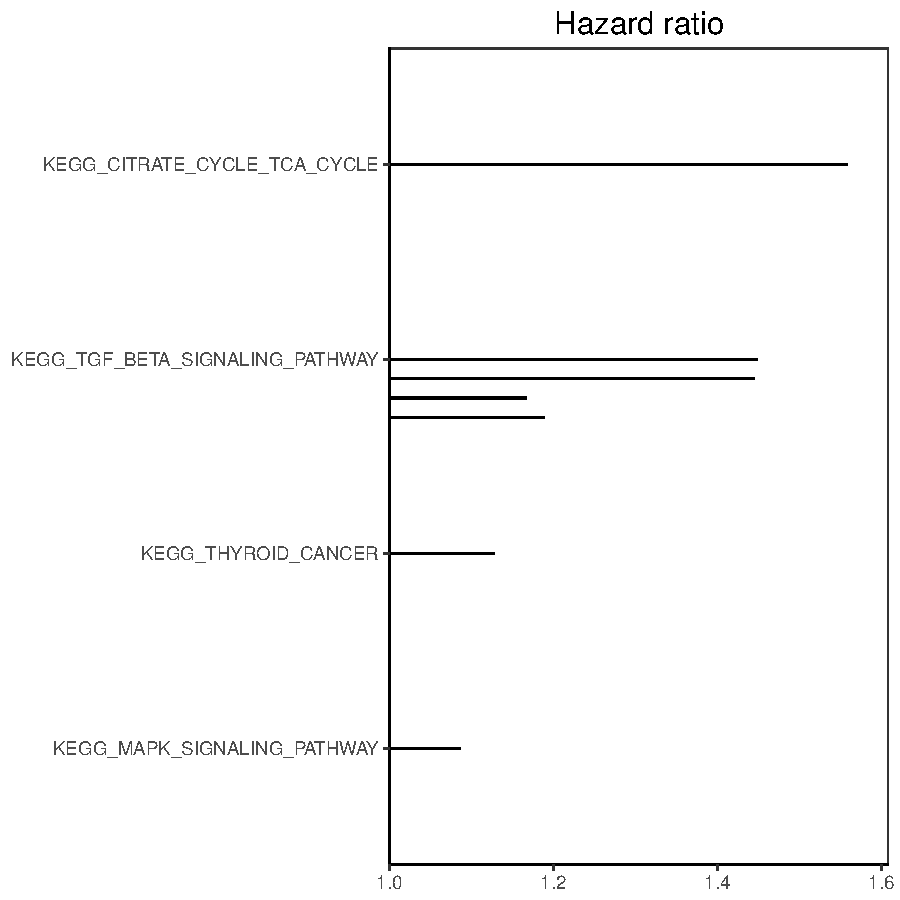
\includegraphics{PICS-example-plot1}
\caption{Hazard ratio (HR) associated with each latent component in the pathways selected by the \texttt{PICS}}
\end{center}
\end{figure}

\section{Risk Group Prediction}
Risk group predictions can be made using the function \texttt{predict()}

\begin{Schunk}
\begin{Sinput}
R> predicted <- predict(path.results)
\end{Sinput}
\end{Schunk}

The function `\texttt{predict}' returns the following output:
(1) risk.index: number of pathways with elevated activity.
(2) riskcat: predicted risk group.
(3) cuts: cut off to determine low, intermediate and high risk group.

\begin{Schunk}
\begin{Sinput}
R> predicted[1:3]
\end{Sinput}
\begin{Soutput}
$risk.index
 [1] 3 4 0 4 2 4 4 0 0 1 4 0 2 3 3 3 0 1 0 2 1 0 1 1 2 2 2 0 0 0 2 0 1 0 0 0 1 0
[39] 4 4 2 4 4 4 4 4 3 4 3 3

$riskcat
 [1] "med"  "high" "low"  "high" "med"  "high" "high" "low"  "low"  "med" 
[11] "high" "low"  "med"  "med"  "med"  "med"  "low"  "med"  "low"  "med" 
[21] "med"  "low"  "med"  "med"  "med"  "med"  "med"  "low"  "low"  "low" 
[31] "med"  "low"  "med"  "low"  "low"  "low"  "med"  "low"  "high" "high"
[41] "med"  "high" "high" "high" "high" "high" "med"  "high" "med"  "med" 

$cuts
[1] 0.00 3.75
\end{Soutput}
\end{Schunk}

\section{Survival Curve}
The predictive performance of \texttt{PICS} method can be presented by Kaplan-Meier curves.
Kaplan-Meier curves of predicted patient subgroups based on the \texttt{PICS} approach can be generated with \texttt{plot()} function with argument \texttt{type="{}KM"{}}.

\begin{Schunk}
\begin{Sinput}
R> plot(path.results, type="KM")
\end{Sinput}
\end{Schunk}

Figure 2 shows the Kaplan-Meier curves of predicted patient subgroups based on the \texttt{PICS} approach. The \texttt{PICS} approach successfully distinguish the high, intermediate and low risk group from each other.

\begin{figure}[tbh]
\begin{center}
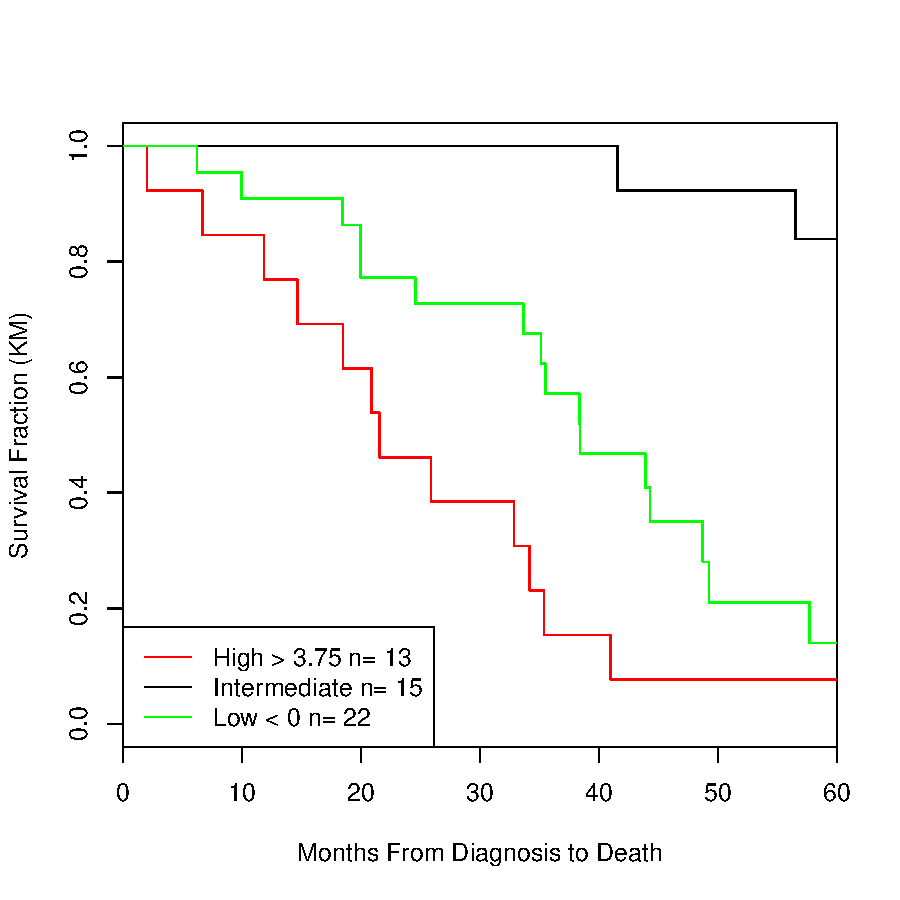
\includegraphics{PICS-example-plot}
\caption{The observed survival curves for patient subgroups identified by the \texttt{PICS}}
\end{center}
\end{figure}

\section{Survival ROC}

The predictive performance of \texttt{PICS} method can be further evaluated based on area under the time dependent receiver operating curve (ROC).
ROC plot can be generated using \texttt{plot()} function with argument \texttt{type="{}ROC"{}}.
\begin{Schunk}
\begin{Sinput}
R> plot(path.results, type="ROC")
\end{Sinput}
\end{Schunk}


\begin{figure}[tbh]
\begin{center}
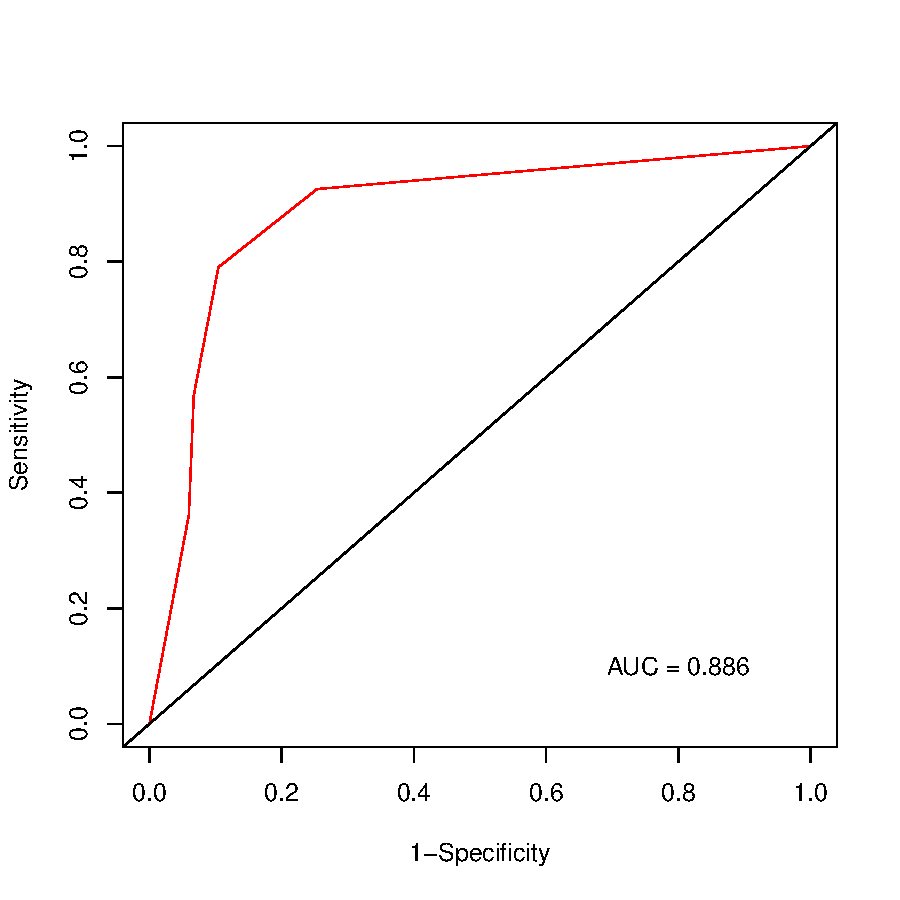
\includegraphics{PICS-example-plot3}
\caption{Time dependent receiver operating curve}
\end{center}
\end{figure}

Figure 3 shows the ROC curves for survival, and for the TCGA data, the area under curve (AUC) associated with the \texttt{PICS} approach was 0.886.


\begin{thebibliography}{99}
\bibitem{PICS} Wei W., Zequn S., Willian S., Zhenning Y., Andrew L., Gary H., Linda K., Dongjun C. (2017), ``PICS: Pathway-guided identification of cancer subtypes''. (submitted).
\bibitem{TCGA} Cancer Genome Atlas Research Network (2011), ``Integrated genomic analyses of ovarian carcinoma''. Nature, 474(7353), 609-615.
\bibitem{SPLS} Bastien, P., Bertrand, F., Meyer, N., Maumy-Bertrand, M. (2014), `` Deviance residuals-based sparse PLS and sparse kernel PLS regression for censored data''. Bioinformatics, 31(3), 397-404.
\bibitem{LASSO} Tibshirani, R. (1997), ``The lasso method for variable selection in the cox model''. Statistics in Medicine, 16(4), 385-395.

\end{thebibliography}

\end{document}
